\documentclass[10pt,a4paper]{article}
\usepackage[T1]{fontenc}
\usepackage[utf8]{inputenc}
\usepackage{lmodern,amsmath,amssymb,graphicx,booktabs,microtype}
\usepackage[margin=22mm]{geometry}
\usepackage[font=small,labelfont=bf]{caption}
\usepackage[numbers,sort&compress]{natbib}
\usepackage[colorlinks=true,allcolors=blue]{hyperref}
\usepackage{placeins}
% Generated; do not edit.
\newcommand{\SharedPlane}{82.918}
\newcommand{\SharedAngle}{0.2726}
\newcommand{\SharedPx}{12.270}
\newcommand{\AlignedPlane}{3.567}
\newcommand{\AlignedAngle}{0.0029}
\newcommand{\AlignedPx}{1.136}
\newcommand{\CentralPlane}{1.820}
\newcommand{\CentralAngle}{0.0015}
\newcommand{\CentralPx}{0.771}
\newcommand{\RayPx}{0.452}
\newcommand{\PistonPct}{97.2}
\newcommand{\CoinDifference}{40.9}
\newcommand{\CoinRayMAD}{17.5}
\newcommand{\CoinCompactMAD}{11.4}
\newcommand{\RigidRigid}{0.015}
\newcommand{\RigidEnriched}{0.019}
\newcommand{\QuadraticRigid}{5.200}
\newcommand{\QuadraticEnriched}{0.022}

\setlength{\parskip}{3pt}
\setlength{\parindent}{1em}
\title{Ray-field residuals as a diagnostic for compact stereo-microscope calibration}
\author{Jean-Fran\c{c}ois Witz\\[3pt]\small Univ. Lille, CNRS, Centrale Lille, LaMcube, Lille, France\\\small\href{mailto:jean-francois.witz@centralelille.fr}{jean-francois.witz@centralelille.fr}}
\date{}
\begin{document}
\maketitle
\begin{abstract}
A flexible camera calibration can describe measured rays accurately while leaving the choice of a compact model unresolved. For stereo microscopy, this distinction matters because geometric constraints introduced during calibration can propagate into surface reconstruction and digital image correlation. We investigate the use of a fitted ray field as a diagnostic reference for model construction, using an existing microscope calibration dataset. Candidate models are fitted to identical ray intersections, while spatial residuals and parameter invariances are examined separately. A shared affine model has a direction residual dominated by its constant component (\PistonPct\,\%). Allowing independent rigid transformations of the two arms reduces the reserved-grid angular RMS from \SharedAngle$^\circ$ to \AlignedAngle$^\circ$. However, a freely fitted central model with 22 coefficients improves both ray agreement and inverse-pixel consistency over the 26-coefficient shared model. The selected reference field is itself central per channel, and two exact parameter invariances prevent interpreting its compact surrogate as a uniquely identified optical assembly. Controlled numerical perturbations distinguish correctable rigid errors from a residual quadratic field. The contribution is a reproducible procedure for testing geometric constraints through ray residuals, with explicit separation between model compression, observational consistency and independent metrological validation. No additional physical measurements are required.
\end{abstract}
\noindent\textbf{Keywords:} stereo microscopy; digital image correlation; camera calibration; ray field; model diagnosis; identifiability.

\section{Introduction}\label{sec:intro}
Stereo digital image correlation (DIC) combines image correspondences with a geometric calibration to estimate three-dimensional shape and displacement. At microscope scales, the optical mapping can contain substantial anisotropy and distortion, and the limited depth of field restricts calibration poses. A small image residual is therefore useful but insufficient to decide whether a camera model expresses the geometry needed for reliable reconstruction. Conversely, a model with coefficients bearing optical names need not provide independently measurable optical parameters.

Microscope calibration is an established problem in experimental mechanics. Schreier, Garcia and Sutton combined distortion estimation and bundle adjustment for stereo light microscopy \citep{schreier2004}. Polynomial mappings offer another practical route: the approach of \citet{soloff1997} underlies the open PYCASO implementation \citep{pycaso2023}. These methods prioritise the mapping required by a measurement system rather than recovery of a lens prescription. Calibration uncertainty also contributes to the uncertainty of DIC results, motivating its analysis beyond the image fit alone \citep{reu2013}.

Representing a camera by its observation lines is not new. Generic camera models and geometric calibration were developed by \citet{grossberg2001,sturm2004}; vision-ray calibration explicitly describes an optical device through its measured rays \citep{bothe2010}. More recent generic calibration includes both central and non-central models and demonstrates downstream biases from restricted camera models \citep{schops2020}. These precedents rule out claiming originality for a pixel-to-ray representation, a two-stage calibration by itself, or the observation that structured residuals indicate model mismatch.

The question addressed here is narrower: how can an already fitted ray field help a DIC practitioner decide which constraints to retain in a compact stereo-microscope model? We use the field as a fixed geometric reference, compare candidate models under the same residual definition, inspect spatial residual components, and test the invariances of their parameters. Residual structure proposes a change in model; an explicit refit determines whether that change helps. This distinction prevents an appealing optical interpretation from replacing a numerical comparison.

The case study revisits an archived PYCASO microscope dataset and an associated Zernike ray-field fit. Starting from a shared affine description, a nearly constant directional mismatch motivates independent arm transformations. A fully fitted central comparator then tests whether the shared construction is actually needed. Controlled perturbations provide a known-answer check of the diagnostic. A stored coin reconstruction illustrates the practical relevance of comparing geometry in a common frame. The resulting contribution is an auditable model-construction procedure and its application to this dataset, rather than a claim of universal superiority or unique identification of a common-main-objective assembly.

\section{Data and geometric reference}\label{sec:data}
\subsection{Existing observations and scope}
The archive contains ten stereo calibration pairs at $2048\times2048$ pixels and a processed observation array of 165 target points per image. The original acquisition belongs to the PYCASO microscope example \citep{pycaso2023}. Recorded stage positions span 2.65--3.35~mm; these stage readings are distinct from the fitted camera-frame board depths. The present analysis starts from the committed arrays and does not acquire or redetect images.

Processing in the archived pipeline combines marker detection, corner completion and thin-plate-spline smoothing. Consequently, the 3300 two-dimensional observations used here include completed and smoothed points. They are not 3300 independent raw detections. All inverse-pixel scores below describe consistency with these processed observations at the archived board poses. They are neither blind test errors nor independently measured camera accuracy. Keeping this scope explicit is essential because smooth completion can conceal systematic corner errors.

The reference is the committed order-$O(0)+d(2)$ Zernike field. Its stored geometry contains 42 scalar coefficients across the two cameras: a constant three-component raw origin and six three-component direction modes per camera. The associated historical calibration count of 57 also includes 15 board-pose variables. Thus, comparisons of ``57 versus 26 parameters'' must distinguish the geometric representation from the pose parameters.

\subsection{Rays, gauge and centrality}\label{sec:rays}
For pixel $p=(u,v)$, camera $c$ defines a line
\begin{equation}
\ell_c(p)=\{O_c(p)+t d_c(p):t\in\mathbb R\},\qquad \|d_c(p)\|=1.
\end{equation}
The reference direction is a normalised pinhole direction plus a Zernike perturbation projected transverse to that direction. The basis is evaluated on the image rectangle mapped inside a unit disk. This is a smooth angular representation, not a measured wavefront. No identification of an individual aberration follows from a Zernike coefficient alone.

A point on a line is not unique: replacing $O$ by $O+\lambda d$ leaves the line unchanged. The implementation selects the transverse representative $O_\perp=O-(O\cdot d)d$. Line comparisons therefore use either intersections with fixed planes or the moment $m=O\times d$, rather than differences between arbitrary origins.

This observation gives an exact centrality check. With a constant raw origin $C_c$, the projected origin is $O_c=C_c-(C_c\cdot d_c)d_c$; hence $C_c=O_c+(C_c\cdot d_c)d_c$ lies on every line of that camera. All nonconstant origin coefficients are exactly zero in the selected cache. Numerical point-to-line distances confirm centrality to floating-point precision. Two different camera centres constitute a stereo pair; they do not establish non-centrality within either camera. Higher-order origin fields remain possible alternatives, but non-centrality is not demonstrated by this reference.

\subsection{Choice of reference complexity}
Table~\ref{tab:orders} retains the archived order sweep in one place. Its scores are local pixel-equivalent ray errors, obtained by multiplying a world-space residual by an approximate local pixel scale. They differ from the numerical inverse-pixel errors introduced in Section~\ref{sec:comparison}. The lowest-order entry is used as a compact diagnostic reference; it is not the minimum-residual entry, and no claim of statistically optimal order is made.

\begin{table}[htbp]\centering
\caption{Archived order sweep. Total coefficients include the 15 pose variables. The last column is a local pixel-equivalent RMS, not numerical reprojection. These historical fits were not rerun for the present comparison.}\label{tab:orders}
\begin{tabular}{rrrr}\toprule
Origin order & Direction order & Total coefficients & Local equivalent (px)\\\midrule
0 & 2 & 57 & 0.470 \\
1 & 2 & 69 & 0.444 \\
0 & 3 & 81 & 0.419 \\
1 & 3 & 93 & 0.412 \\
2 & 3 & 111 & 0.409 \\
1 & 4 & 123 & 0.412 \\
2 & 4 & 141 & 0.410 \\
\bottomrule
\end{tabular}

\end{table}

\section{Residual-guided model construction}\label{sec:method}
\subsection{Comparable ray-space objectives}\label{sec:comparison}
A line intersects a plane of depth $z$ at the transverse coordinate
\begin{equation}
q_z(O,d)=O_{xy}+\frac{z-O_z}{d_z}d_{xy}.
\label{eq:plane}
\end{equation}
Two distinct planes identify the line when $d_z\ne0$. We fit every candidate to the same two-plane objective,
\begin{equation}
E(\beta)=\sum_{c,p,z}\|q_z(\ell_c(p;\beta))-q_z(\ell_c^{\rm ref}(p))\|^2,
\qquad z\in\{50,80\}\;\mathrm{mm}.
\label{eq:objective}
\end{equation}
The training grid contains $17\times13$ pixels per camera, giving 1768 scalar residuals. Only the two nontrivial coordinates are included; the identically zero depth residual is omitted. A linear least-squares loss and identical weights are used for all candidates. A separate $32\times24$ grid uses cell midpoints and shares no pixels with the training grid. Reported ray RMS is the square root of the mean squared two-dimensional intersection distance over both cameras and planes.

The reserved grid evaluates compression of a fixed fitted field between training pixels. It is not a holdout of physical observations. The two plane depths control the relative importance of angular and positional mismatch; evaluating an existing line at these depths adds no measured depth range. In particular, the 30~mm separation of the comparison planes is not a 30~mm calibration validation.

We also report the RMS angle between model and reference directions. For image-space consistency, we numerically solve $q_{X_z}(\ell_c(p_{\rm pred}))=X_{xy}$ at each archived board point and compare $p_{\rm pred}$ with the processed observation. The same board poses are held fixed for all candidates, including the reference. This inverse uses the local two-dimensional Jacobian of Equation~\ref{eq:plane}; the supplementary material gives the algorithm and closure check. No global conversion factor is used to turn ray errors into pixels.

\subsection{Candidate constraints and residual hypotheses}\label{sec:candidates}
The first candidate is the existing shared affine stereo construction. For each arm, its unnormalised direction has a common chief-ray component with per-channel horizontal and vertical slopes. Its origin is a symmetric baseline point plus an affine pupil-shear term. In compact notation,
\begin{align}
\widetilde d_c(p)&=(s_c\sin\theta+a_{xc}\widetilde u,\ d_y+a_{yc}\widetilde v,\ \cos\theta),\\
O_c(p)&=(-s_c b/2+\rho_x\widetilde u,\ \rho_y\widetilde v,\ WD-f),
\end{align}
where $s_L=1$, $s_R=-1$, $\widetilde u=(u-c_x)h/f_a$ and $\widetilde v=(v-c_y)h/f_a$. Directions are normalised. The pixel-pitch convention is $h=0.0055$~mm. This vector contains 14 stored coefficients; the code's historical class name includes ``telecentric'', but the equations do not impose strictly parallel object-space chief rays. We therefore use the descriptive name \emph{shared affine model}.

A nearly constant directional residual suggests testing an arm-frame correction before adding more spatial modes. The second candidate applies an independent rigid transformation to each arm,
\begin{equation}
O'_c=R_cO_c+t_c,\qquad d'_c=R_cd_c,
\end{equation}
giving 26 stored coefficients. Rotations and translations affect line directions and positions jointly; their benefit is assessed by refitting, not by assigning a physical cause to a residual image. Four starting arm configurations are used for this fit. The optimisation bounds and starts are recorded in the executable analysis.

The third candidate removes shared optical constraints and fits one general central projective camera per channel. With normalised image coordinates $(x,y)$,
\begin{equation}
O_c=C_c,\qquad d_c=\operatorname{normalise}\left[
 a_{0c}+a_{1c}x+a_{2c}y,\ b_{0c}+b_{1c}x+b_{2c}y,\ 1+c_{1c}x+c_{2c}y\right]^T.
\label{eq:central}
\end{equation}
Its three centre coordinates and eight directional coefficients give 11 coefficients per channel, or 22 in total. This is a freely fitted central comparator, including skew and unequal directional scales, rather than a fixed nominal pinhole. A least-squares centre estimate and linear projective-direction fit initialise its refinement. It does not include Brown distortion, so it is not intended to exhaust the possible central models.

\subsection{Spatial decomposition and identifiability}\label{sec:diagnosis}
On the reserved grid, the vector residual $\Delta d=d_{\rm model}-d_{\rm ref}$ is projected onto nested constant, linear and quadratic polynomial spaces. A QR factorisation of the sampled design matrix $[1,x,y,x^2,y^2,xy]$ gives an orthonormal discrete basis. Energies are summed over vector components and cameras. The remainder is the residual outside this quadratic space. The resulting fractions sum to unity; they do not rely on continuous Zernike orthogonality over a square sampling grid. The constant component is the analogue of a piston term, but is a geometric direction residual rather than optical path difference.

This decomposition is a diagnostic, not a classifier of optical components. A constant direction offset can arise from an arm rotation, a coordinate convention or another parameter compensation. A linear pattern can arise from scale or cross-axis mismatch. Candidate explanations are tested through the corresponding change in the model and the reserved-grid residual. The decomposition itself cannot establish which physical element produced the discrepancy.

Parameter invariances are checked independently. In the shared model, replacing $(f,WD)$ by $(f+\delta,WD+\delta)$ leaves the origin unchanged when $f_a$ is independent. Multiplying $f_a$, every slope and every shear coefficient by the same factor also leaves all rays unchanged. We fix $f$ and $f_a$ to the declared convention of 62.2089148981~mm during the new fits. This removes these two exact directions of redundancy without asserting a measured focal length. Remaining singular directions are reported from the column-normalised residual Jacobian.

Pose coupling is a separate issue. For optical variables $\beta$ and poses $\eta$, the local information remaining after pose elimination is the Schur complement $S=H_{\beta\beta}-H_{\beta\eta}H_{\eta\eta}^{+}H_{\eta\beta}$, after appropriate gauge fixing and scaling. Fitting to a fixed field removes pose variables from the second optimisation; it does not recover optical information absent from the original observations. Detailed Schur regularisation is therefore kept outside the principal contribution.

\section{Results}\label{sec:results}
\subsection{From a constant residual to a better compact model}
The shared affine model leaves an angular RMS of \SharedAngle$^\circ$ on the reserved grid, with \PistonPct\,\% of direction-residual energy in the constant component. Adding independent arm transformations lowers the angular RMS to \AlignedAngle$^\circ$ and the two-plane RMS from \SharedPlane~$\mu$m to \AlignedPlane~$\mu$m. The four starts converge to essentially the same objective value, supporting this as a stable local comparison under the stated bounds.

\begin{figure}[htbp]\centering
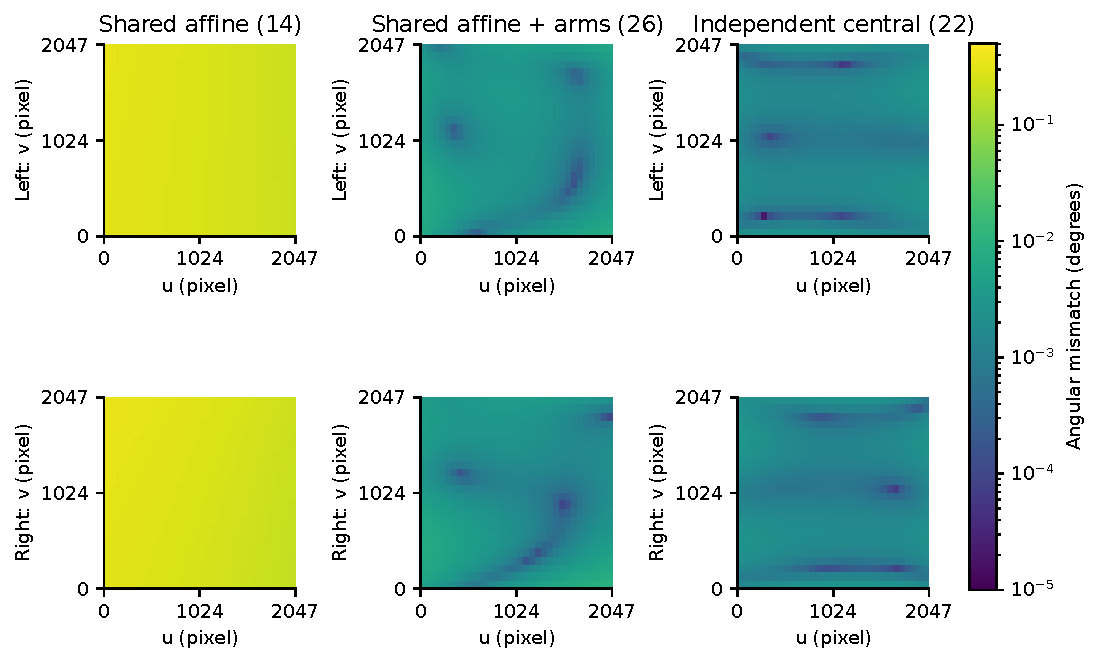
\includegraphics[width=.96\linewidth]{figures/diagnostic_residuals.pdf}
\caption{Recomputed angular residuals against the same reference field, at pixels excluded from the ray-space fit. All six maps share one logarithmic colour scale. Independent arm transformations remove most of the shared-model mismatch; the freely fitted central comparator reduces it further.}\label{fig:residuals}
\end{figure}

\begin{table}[htbp]\centering\small
\caption{New comparison with identical ray-space objectives. Ray scores are two-plane XY RMS in $\mu$m. The last column is numerical inverse-pixel RMS at the same archived board poses, using processed fitted observations. It is not a blind validation score. Counts in parentheses are stored geometric coefficients.}\label{tab:models}
\begin{tabular}{lrrrr}\toprule
Model & Training & Reserved & Angle ($^\circ$) & Inverse (px)\\\midrule
Shared affine (14) & 83.798 & 82.918 & 0.2726 & 12.270 \\
Shared affine + arms (26) & 4.031 & 3.567 & 0.0029 & 1.136 \\
Independent central (22) & 2.127 & 1.820 & 0.0015 & 0.771 \\
\bottomrule
\end{tabular}

\end{table}

The central comparator reaches \CentralPlane~$\mu$m and \CentralAngle$^\circ$, with fewer stored coefficients than the 26-coefficient construction. Its inverse-pixel RMS is \CentralPx~px, compared with \AlignedPx~px for the latter. The reference field itself gives \RayPx~px under the same numerical inversion. These values differ from the older local pixel-equivalent scores because the metric and fitted compact models have changed. Table~\ref{tab:models} is the internally consistent comparison used here.

The result supports residual-guided model revision, but not rejection of central cameras. The reference is central by construction, and a freely fitted central model is the strongest compact candidate in this experiment. Accordingly, the 26-coefficient shared model is an informative intermediate hypothesis, not the preferred final representation on these criteria. The benefit of the ray field is precisely that it allows this constraint to be questioned before attaching a physical interpretation to it.

\begin{figure}[htbp]\centering
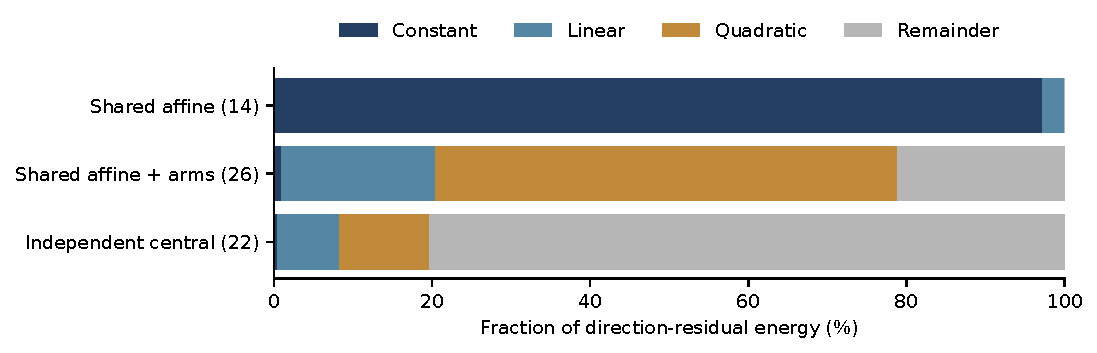
\includegraphics[width=.92\linewidth]{figures/diagnostic_modes.pdf}
\caption{Discrete orthogonal decomposition of direction-residual energy. Fractions describe structure within each residual and must be read with its absolute amplitude in Table~\ref{tab:models}. A large remainder fraction for a much smaller residual is not evidence of worse calibration.}\label{fig:modes}
\end{figure}

The corrected shared model leaves a substantial quadratic component, whereas the smaller central residual has a larger relative remainder. This does not establish a particular aberration: each component depends on the reference basis, the sampled region and the candidate constraints. Nor does it imply that adding arbitrarily high orders is warranted. The reference already carries processing error and the uncertainty of its calibration; further compression accuracy must be judged against that uncertainty.

\subsection{Controlled diagnostic check}\label{sec:simulation}
To test whether the proposed reasoning can distinguish specified failure modes, we generate rays from the fitted central comparator and add known arm perturbations. In one case, the truth is a rigid transform only. In the other, the same type of transform is combined with quadratic direction perturbations $2\times10^{-4}(x^2-1/3)$ and $-1.5\times10^{-4}(y^2-1/3)$ in the first two components before normalisation. Independent Gaussian perturbations of standard deviation $2\times10^{-6}$ are added to each direction component at the training pixels. Twenty seeded realisations are run per case; rotation-vector components and translations have standard deviations 0.008~rad and 0.15~mm, respectively.

Both a rigid correction and a rigid-plus-quadratic correction are fitted to the noisy training rays. Evaluation uses noise-free truth at the reserved pixels. For rigid-only truth, median ray RMS is \RigidRigid~$\mu$m for the rigid fit and \RigidEnriched~$\mu$m for the enriched fit. With an added quadratic field, the corresponding values are \QuadraticRigid~$\mu$m and \QuadraticEnriched~$\mu$m. Thus, extra spatial terms help when the specified mismatch contains those terms and do not improve this rigid-only control.

\begin{figure}[htbp]\centering
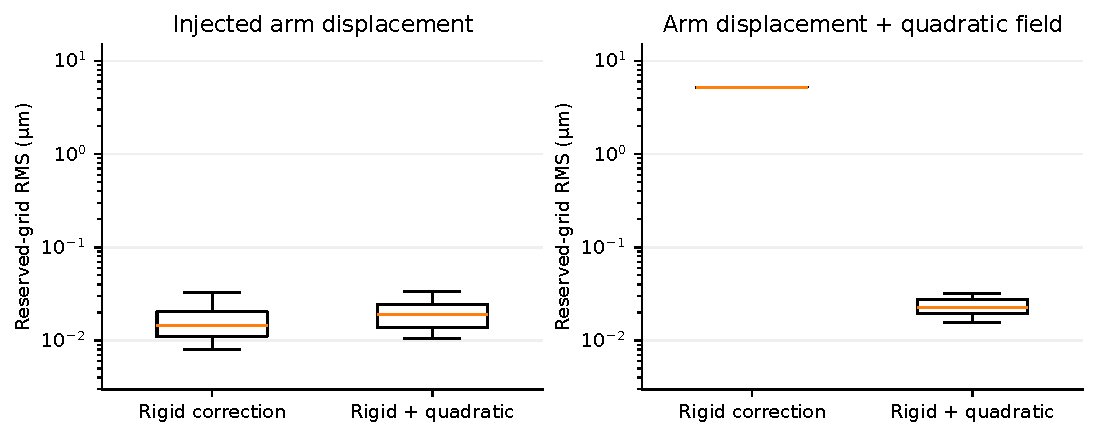
\includegraphics[width=.95\linewidth]{figures/diagnostic_simulation.pdf}
\caption{Controlled perturbation experiment, twenty realisations per case. Boxes show quartiles and medians of reserved-grid error against known noise-free rays. The two panels share the logarithmic vertical scale. This is a check of the geometric diagnostic under specified perturbations, not an experimental validation of the microscope or a new image-correlation test.}\label{fig:simulation}
\end{figure}

These are deliberately controlled tests with perturbations represented by the candidate model. They establish correct behaviour for the stated cases, not general identification of unknown aberrations. The ability to distinguish smaller mixed perturbations, or perturbations outside the chosen basis, remains to be established. The numerical noise level is a simulation input, not an estimate of the camera's measurement noise.

\subsection{Parameter interpretation and a specimen illustration}\label{sec:specimen}
Numerical evaluation confirms the two exact parameter invariances: a simultaneous 10~mm shift of $f$ and $WD$, and a 20\,\% rescaling of angular scale, slopes and shears, preserve two-plane intersections to machine precision. Optical labels in the parameter vector therefore do not provide separate physical measurements of these quantities. The fitted 26-coefficient model also retains very small singular values after fixing the two explicit gauges. Counting its stored coefficients as 26 independently identified optical degrees of freedom would be misleading.

For the specimen illustration, the archive provides two coin surfaces reconstructed from the same correspondences with an earlier ray-field model and an earlier compact model. These surfaces are not outputs of the new fits in Table~\ref{tab:models}. We use their common validity mask of 1,943,070 points, take a deterministic subsample of 100,000, align the compact cloud to the ray-field cloud by one rigid transformation and subtract a best-fit plane from each height field in the common coordinates. The median three-dimensional difference after alignment is \CoinDifference~$\mu$m. Detrended height MAD is \CoinRayMAD~$\mu$m and \CoinCompactMAD~$\mu$m, respectively.

\begin{figure}[htbp]\centering
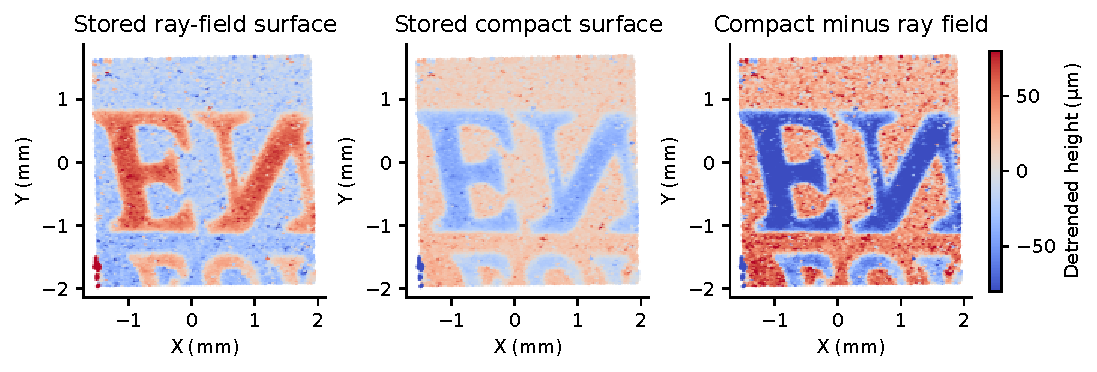
\includegraphics[width=.98\linewidth]{figures/diagnostic_coin.pdf}
\caption{Reanalysis of two archived coin surfaces, using a common point mask, one rigid alignment and explicit planar detrending. The residual relief differs even after this frame correction. Values quantify disagreement between reconstructions; neither surface is an independent reference.}\label{fig:coin}
\end{figure}

A smaller whole-surface or detrended MAD is not evidence of higher accuracy: it can represent reduced relief as well as reduced noise. Similarly, a small gap between left and right rays establishes internal intersection consistency, not correctness of the reconstructed height. The published PYCASO study contains specimen comparisons, but the numerical independent height reference is not part of the inspected input archive. The coin example therefore motivates checking geometric consequences without assigning an accuracy ranking to these surfaces.

\section{Discussion}\label{sec:discussion}
The main practical value is a sequence of falsifiable geometric questions. Does a candidate preserve the observed lines? Which spatial component dominates its error? Does releasing the corresponding constraint improve agreement at unsampled pixels? Does a simpler independently fitted camera explain the same field? Finally, are changes in named optical parameters observable at all? These questions are useful to DIC users because they expose model restrictions before those restrictions are interpreted as specimen geometry.

The result also limits the optical conclusion. The observed improvement from independent arm transformations shows that the initial shared constraints are too restrictive for this reference. It does not uniquely identify arm misalignment, prove object-space telecentricity or recover a lens prescription. The invariances prevent using fitted working distance and focal length to contradict the microscope designation in the original experimental publication. A physical identification claim would require independent constraints on the relevant optical quantities and discrimination between competing architectures.

We deliberately avoid an evidential ranking of optical families through the old BIC values. The historical implementation duplicated the same full-grid residual block for one shared-model fit and used differently constrained central baselines. Moreover, samples from a fitted polynomial ray field are correlated, and adding grid pixels does not create new experimental observations. Parameter gauges further complicate the model dimension entering a likelihood penalty. Correcting a residual-count bug is necessary, but cannot by itself turn a ray-space approximation score into evidence for an optical family. The new comparison reports directly interpretable residuals, declared coefficient counts and a freely fitted central alternative.

For DIC, the distinction between reference compression and calibration validation is decisive. The reserved-grid experiment tests how well a compact mapping approximates the chosen ray field. It does not test the ray field's error relative to the actual instrument, and the processed-corner inverse score reuses fitted observations. The present work consequently supports a calibration diagnostic and software procedure. It does not quantify strain accuracy, replace uncertainty propagation or establish performance across instruments, zoom settings or calibration depths.

Several extensions remain possible without new physical measurements. Existing raw images could support a common detector-only comparison that excludes completed points, with entire acquisition frames held out before smoothing and fitting. Propagating perturbations through that complete pipeline would estimate the sensitivity of the diagnostic to corner processing. Synthetic rigid specimen motions could quantify false strain from a fixed calibration mismatch, provided the generating geometry is varied independently of the fitted family. These are distinct experiments; the controlled ray perturbations reported here must not be relabelled as any of them.

The broader use is as a calibration audit: inspecting model constraints, detecting changes between repeated calibration files, and choosing a compact surrogate when the generic reference is expensive to deploy. Such uses depend on the quality of the reference itself. Residual maps are most informative when accompanied by their absolute amplitude, a declared coordinate convention and an explicit uncertainty or repeatability analysis. Their spatial appearance alone cannot supply those missing elements.

\section{Conclusion}
An existing fitted ray field can guide compact model construction through comparable line residuals, spatial decomposition and invariance checks. In this microscope example, the dominant constant directional residual motivates independent arm transformations and the refit substantially reduces the mismatch. A freely fitted 22-coefficient central model performs better still, showing why the diagnostic must be allowed to reject the original shared optical constraints. The selected reference is central per camera, and exact parameter gauges preclude unique physical interpretation of the shared model. The supported contribution is a reproducible diagnostic for calibration modelling; independent surface and strain accuracy remain outside the evidence supplied by these data.

\FloatBarrier
\section*{Data and code availability}
Code, processed observations, reference rays and analysis outputs are provided in \href{https://github.com/jeffwitz/StereoComplex/tree/codex/cmo-diagnostic-paper/paper/cmo}{StereoComplex, branch codex/cmo-diagnostic-paper}. The analysis records SHA-256 hashes of its inputs and the source base commit. The supplementary document specifies the rerun commands and the status of historical results. Raw PYCASO data are available from \url{https://github.com/LaboratoireMecaniqueLille/Pycaso}. No archival DOI is claimed for this working version.
\bibliographystyle{unsrtnat}
\bibliography{references}
\end{document}
